\chapter{Details}
%------------------------------------------------------------------------------
% Elaboration
%20 pages. Details of the Dependency Analysis Plugin (DAP. Describe the DAP-DB and %DAP-INCQUERY solution too. 
%------------------------------------------------------------------------------

\section{Infrastructure at CERN controls systems}

\subsection{Used tools}
- Describe, how a typical developer works at CERN BE-CO 
- Tools: SVN, Eclipse, Common Build, JIRA, etc. % check this at some papers of vito.

\subsection{Development workflow}
- Original idea comes from the typical development workflow lifecycle at CERN
control systems. %Insert one-by one the explanation form my thesis1 report.

%------------------------------------------------------------------------------
% Bytecode analysis 
%------------------------------------------------------------------------------
\section{Bytecode analysis}

\subsection{Anatomy of class files}
- Describe how the class is constructed.
- List what kind of dependencies are extracted from this system. 

\subsection{Execution of dependency discovery}
- Sequence, how the dependency analysis works. 
- Summarize what should be found if execute the analysis in the example

\begin{figure}[htb]
   \center   
   \caption{Sequence of bytecode analysis} 
   \label{fig:analization.pdf}  
     \resizebox{0.7\linewidth}{!}{
      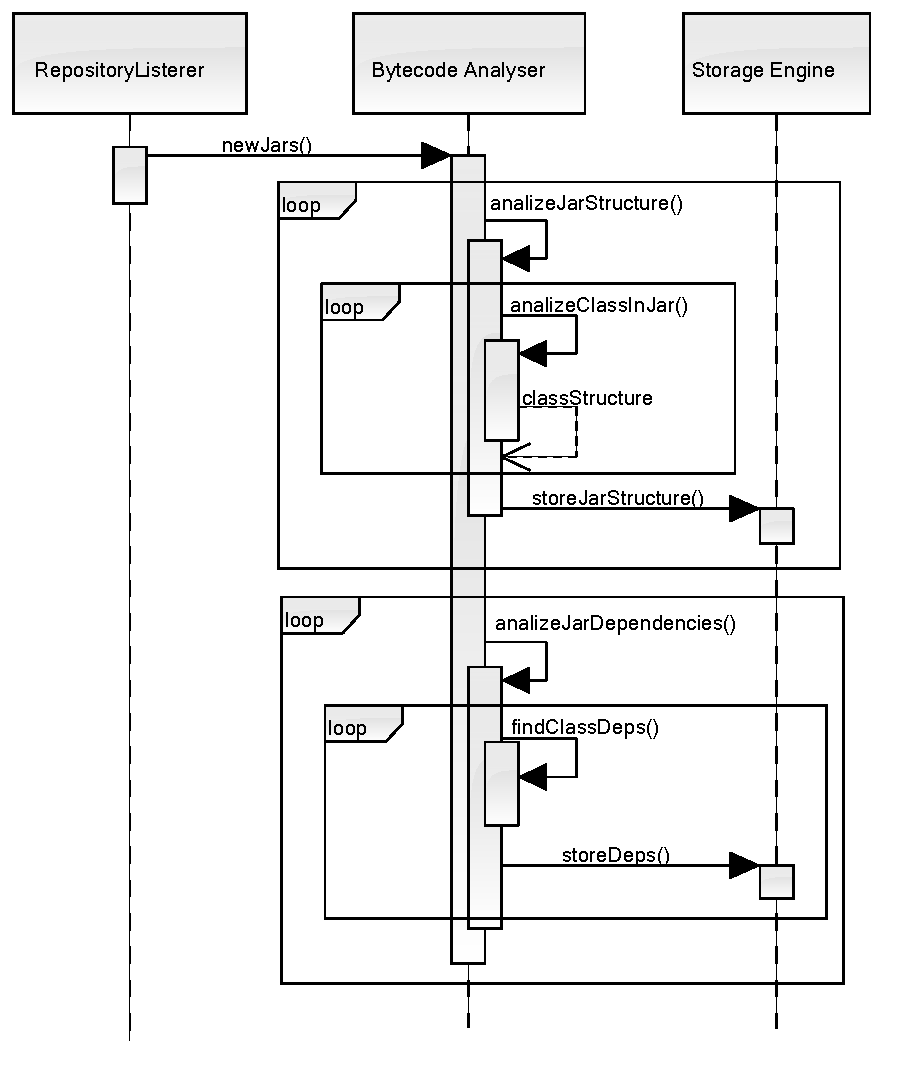
\includegraphics{figures/analization.pdf}
      } 
\end{figure}

%------------------------------------------------------------------------------
% Persistence
%------------------------------------------------------------------------------
\section{Persisting dependencies} 
- describe the saved domain model.
- describe the how the operations work:
 * store structure
 * find and insert dependencies
- introduce different implementation 
- the result 

\section{Direct queries}
- Explain eclipse plugin; ui contribution.
- Simple workflow: right click on source code->jdt resolves it as a
class-method-field-> fully qualify it -> sends the query for the server process
-> the process returns the incoming dependencies depending the passed type. ->
the result is visualized in a view.
- Show it on the example: what if the developer wants to change the the
signature of a service function OR what if he wants to change the name of the
name of the default provider name.

\section{Repository EMF model}
% bonus: retrieve the model to the client

\section{Creation of workspace EMF model}
- Java Model representation in Eclipse. 
- Dependency search in Eclipse.
- EMF model generation:
 * How to obtain the structure 
 * How to obtain internal dependency environment
 * and how to listen to changes.

\section{Pattern matching}
- Mention again that the source code and the repository contains the same information. (+svn tags)
- How to obtain more precise information.
- The repository model. 
- Describing the queries.
* joining the two implementation. 
* incoming dependencies
* impact analysis
  * added and removed methods
  * removed methods
  * changed methods: the outgoing dependency set has new elements, which does not exist in the repo model. 
-  Show it on the example.
